\documentclass[a4paper, 12pt]{article}
  
\usepackage{algorithm}
\usepackage{amsmath}
\usepackage{amssymb}
\usepackage{multicol} 
\usepackage{color, colortbl}
\usepackage{tikz}

\definecolor{Gray}{gray}{0.9}
\definecolor{LightCyan}{rgb}{0.70,1,1}
\definecolor{OliveGreen}{rgb}{0,0.6,0}

\setlength{\parindent}{0pt}
\newcommand{\norm}[1]{\left\lVert#1\right\rVert}

\title{Notes on Vectors}
%comment comment comment
\begin{document} 
\textbf{Linear Equation}
is equation where $n$ variables $x_1, x_2, ..., x_n$  can be expressed in the form
$a_1x_1 + a_2x_2 + ... + a_nx_n = b $ \\
where $a_1, a_2, ..., a_nx_n$ and $b$ are constants, and $a's$  are not all zero.
\\
\\
\textbf{System of linear equations} or \textbf{linear system} is a finite test of 
linear equations.The variables are called \textbf{unknowns}
\\
\\
\textbf{Solution} of a linear system with $n$ unknonws $x_1, x_2, ... , x_n$ is 
a sequance of $n$ numbers  $s_1, s_2, ... s_n$ for which the substitution
$x_1 = s_1, x_2 = s_2, ..., x_n = s_n$
makes each equation a true statement.
\\
\\
\textit{Every system of linear equations has zero, one or infinitely many solutions.
There are no other possibilities.}
\\
\\
\textbf{Consistent} linear system is the one that has at least one solution.
They are two equations in this system,  one solution of infinitely many.
\\
\\
\textbf{Inconsistent} linear system is the one that has no solutions.
\\
\\ 
\textbf{Matrix} is rectangular array of numbers.
\\
\\
\textbf{Size of A Matrix} is described in terms of number of rows(horizontal lines)
and columns(vertical lines). For example matrix with 3 rows and 2 columns have size
3 by 2 (written 3 x 2)
\\
\\
\textbf{Augmented Matrix} is a matrix obtained by appending the columns of 
two given matrices.\\
Given the matrices A and B, where
$$
A =
\begin{bmatrix}
1 && 3 && 2 \\
2 && 0 && 1 \\
5 && 2 && 2
\end{bmatrix}
\quad
, B = 
\begin{bmatrix}
4 \\
3 \\
1
\end{bmatrix}
$$
\\
the augmented matrix $(A|B)$ is written as
$$
(A|B) = 
\begin{bmatrix}
1 & 3 & 2 & 4\\
2 & 0 & 1 & 3\\
5 & 2 & 2 & 1
\end{bmatrix}
$$
\\
Augmented Matrix can be used to represent sytem equations.
For example :
\begin{multicols}{2}
\begin{align*}
x_1 + x_2 + 2x_3 &= 9 \\
2x_1 + 4x_2 - 3x_3 &= 1 \\
3x_1 + 6x_2 - 5x_3 &= 0\\
\end{align*}
\break
\[ \left[ {\begin{array}{cccc}
1 & 1 & 2 & 9 \\
2 & 4 & -3 & 1 \\
3 & 6 & -5 & 0
\end{array}} \right] \]
\end{multicols}

\textbf{Elementary Row Operations}
The basic method for solving a linear system is to perform appropiate 
algebraic operations on the system that do not alter the solution set 
and that produce a succession of increasingly simple system, until a 
point is reached where it can be ascertained whether the system is 
consistent, and if so, what its solutions are. Typically, the algebraic
operations are as follows:
\begin{enumerate}
\item Multiply an equation through by a nonzero constant
\item Interchange two equations
\item Add a constant times of one equation to another 
\end{enumerate}

Since the rows (horizontal lines) of an augmented matrix correspond
to the equations in the associated system, these three operations 
correspond to the following operation on the rows of the augmented
matrix 
\begin{enumerate}
\item Multiply a row through by a nonzero constant
\item Interchange two rows
\item Add a constant times of one row to another 
\end{enumerate}

\begin{multicols}{2}
\begin{align*}
x + y + 2z &= 9 \\
2x + 4y - 3z &= 1 \\
3x + 6y - 5z  &= 0\\
\end{align*}
\break
\[ \left[ {\begin{array}{cccc}
1 & 1 & 2 & 9 \\
2 & 4 & -3 & 1 \\
3 & 6 & -5 & 0
\end{array}} \right] \]
\end{multicols}

\begin{multicols}{2} 
Add -2 times the first equation to all equation
\break
Add -2 times the first row to all row
\end{multicols}

\begin{multicols}{2}
\begin{align*}
-x  -y - 2z &= -9 \\
2y - 7z &= -17 \\
x + 4y - 9z  &= -18\\
\end{align*}
\break
\[ \left[ {\begin{array}{cccc}
-1 & -1 & -2 & -9 \\
0 & 2 & -7 & -17 \\
1 & 4 & -9 & -18 
\end{array}} \right] \]
\end{multicols} 

\begin{multicols}{2} 
Add the first equation the third equation
\break
Add the first row to the third row
\end{multicols}

\begin{multicols}{2}
\begin{align*}
-x  -y - 2z &= -9 \\
2y - 7z &= -17 \\
3y - 11z  &= -27\\
\end{align*}
\break
\[ \left[ {\begin{array}{cccc}
-1 & -1 & -2 & -9 \\
0 & 2 & -7 & -17 \\
0 & 3 & -11 & -27 
\end{array}} \right] \]
\end{multicols} 

\begin{multicols}{2} 
Add -1 of the third equation the second equation
\break
Add -1 of the third row to the second row
\end{multicols} 

\begin{multicols}{2}
\begin{align*}
-x  -y - 2z &= -9 \\
-y + 4z &= 10 \\
3y - 11z  &= -27\\
\end{align*}
\break
\[ \left[ {\begin{array}{cccc}
-1 & -1 & -2 & -9 \\
0 & -1 & +4 & 10 \\
0 & 3 & -11 & -27 
\end{array}} \right] \]
\end{multicols} 

\begin{multicols}{2} 
Add -1 of the second equation the first equation
\break
Add -1 of the second row to the first row
\end{multicols} 

\begin{multicols}{2}
\begin{align*}
-x +  0y  - 6z &= -19 \\
-y + 4z &= 10 \\
3y - 11z  &= -27\\
\end{align*}
\break
\[ \left[ {\begin{array}{cccc}
-1 & 0 & -6 & -19 \\
0 & -1 & 4 & 10 \\
0 & 3 & -11 & -27 
\end{array}} \right] \]
\end{multicols} 

\begin{multicols}{2} 
Add 3 times of the second equation the third equation
\break
Add 3 times  of the second row to the third row
\end{multicols} 

\begin{multicols}{2}
\begin{align*}
-x +  0y  - 6z &= -19 \\
-y + 4z &= 10 \\
z  &= 3
\end{align*}
\break
\[ \left[ {\begin{array}{cccc}
-1 & 0 & -6 & -19 \\
0 & -1 & 4 & 10 \\
0 & 0 & 1  & 3 
\end{array}} \right] \]
\end{multicols} 

\begin{multicols}{2} 
Add 6 times of the third equation the first equation
\break
Add 6 times of the third row to the first row
\end{multicols} 

\begin{multicols}{2}
\begin{align*}
-x &= -1 \\
-y + 4z &= 10 \\
z  &= 3\\
\end{align*}
\break
\[ \left[ {\begin{array}{cccc}
-1 & 0 & 0  & -1 \\
0 & -1 & 4 & 10 \\
0 & 0 & 1  & 3 
\end{array}} \right] \]
\end{multicols} 

\begin{multicols}{2} 
Add -4 times of the third equation the second equation
\break
Add -4 times of the third row to the second row
\end{multicols}

\begin{multicols}{2}
\begin{align*}
-x &= -1 \\
-y &= -2 \\
z  &= 3\\
\end{align*}
\break
\[ \left[ {\begin{array}{cccc}
-1 & 0 & 0  & -1 \\
0 & -1 & 0 & -2 \\
0 & 0 & 1  & 3 
\end{array}} \right] \]
\end{multicols} 

\begin{multicols}{2} 
Multiply -1 times for each equation 1 and 2
\break
Multiply -1 times for each row 1 and 2
\end{multicols}


\begin{multicols}{2}
\begin{align*}
x &= 1 \\
y &= 2 \\
z  &= 3\\
\end{align*}
\break
\[ \left[ {\begin{array}{cccc}
1 & 0 & 0  & 1 \\
0 & 1 & 0 & 2 \\
0 & 0 & 1  & 3 
\end{array}} \right] \]
\end{multicols} 

\textbf{Echelon Forms and Reduced Echelon Forms}
\begin{enumerate}
\item If row does not consists of entirely zeroes, then the first nonzero 
      number in the row is a 1. This is called a \textit{leading 1}.
\item It there are any rows that consist entirely of zeroes, the they are 
      grouped together a the bottom of the matrix.
\item In any two succesive rows that do not consist entirely of zeros, the 
      leading 1 in the lower row occurs farther to the right the the 
      leading 1 in the higher row.
\item Each column that contains a leading 1 has zeroes everywhere else in
      the column.
\end{enumerate}
1 to 3 is property of  \textit{row echelon form}, meanwhile 1 to 4 is 
property of \textit{reduced row echelon form}.
\\
\\
Example of Reduced Echelon Form
$$
\begin{bmatrix}
1 && 0 && 0 && 4 \\
0 && 1 && 0 && 7 \\
0 && 0 && 1 && -1 \\
\end{bmatrix}
\quad
\begin{bmatrix}
1 && 0 && 0 \\
0 && 1 && 0 \\
0 && 0 && 1 \\
\end{bmatrix}
\quad
\begin{bmatrix}
0 && 1 && -2 && 0 && 1 \\
0 && 0 && 0 && 1 && 3  \\
0 && 0 && 0 && 0 && 0  \\
0 && 0 && 0 && 0 && 0  \\
\end{bmatrix}
$$

Example of Echelon Form but not Reduced
$$
\begin{bmatrix}
1 && 4 && -3 && 7 \\
0 && 1 && 6 && 2 \\
0 && 0 && 1 && 5
\end{bmatrix}
\quad
\begin{bmatrix}
1 && 1 && 0 \\
0 && 1 && 0 \\
0 && 0 && 0
\end{bmatrix}
\quad
\begin{bmatrix}
0 && 1 && 2 && 6 && 0 \\
0 && 0 && 1 && -1 && 0 \\
0 && 0 && 0 && 0 && 1
\end{bmatrix}
$$
\\
\\
\textbf{General Solutions}. If a linear system has infinitely many solutions,
then a set of parametric equations from which all solutions can be obtained
by assigning numerical values to the parameters is called 
\textbf{general solution} to the system.
\\
\\
\textbf{Elimination Procedure} is steps that can be used to reduce matrix to 
reduced echelon form
\\
\\
\textbf{Gauss-Jordan Elimination}.
\[ \left[ {\begin{array}{cccccc}
0 & 0 & -2  & 0 & 7 & 12 \\
2 & 4 & -10 & 6 & 12 & 28 \\
2 & 4 & -5 & 6 & -5 & -1
\end{array}} \right] \]

\begin{enumerate}
\item Locate the leftmost column that does not consist entirely zeros
\[ \left[ {\begin{array}{cccccc}
0 & 0 & -2  & 0 & 7 & 12 \\
\rowcolor{Gray}
2 & 4 & -10 & 6 & 12 & 28 \\
2 & 4 & -5 & 6 & -5 & -1
\end{array}} \right] \]
\item Interchange the top row with another row, if necessary, to bring 
a nonzeor entry to the top of the column found in 1
\[ \left[ {\begin{array}{cccccc}
\rowcolor{Gray}
2 & 4 & -10 & 6 & 12 & 28 \\
\rowcolor{Gray}
0 & 0 & -2  & 0 & 7 & 12 \\
2 & 4 & -5 & 6 & -5 & -1
\end{array}} \right] \]
\item If the entry that is now at the top of the column found in 1 is a,
multiply the first row by $1/a$ in order to introduce a leading 1.
\[ \left[ {\begin{array}{cccccc}
\rowcolor{Gray}
1 & 2 & -5 & 3 & 6 & 14 \\
0 & 0 & -2  & 0 & 7 & 12 \\
2 & 4 & -5 & 6 & -5 & -1
\end{array}} \right] \]
\item Add a suitable multiples of the top row to the rows below so that
all entries below the leading 1 becomes zeros
\[ \left[ {\begin{array}{cccccc}
1 & 2 & -5 & 3 & 6 & 14 \\
0 & 0 & -2  & 0 & 7 & 12 \\
\rowcolor{Gray}
0 & 0 & 5 & 0 & -17 & -29
\end{array}} \right] \]
\item Now cover the top row in the matrix and begina again with step 1
applied to the submatrix that remains. Continue in this way untuk the
entire matrix in row echelon form
\[ \left[ {\begin{array}{cccccc}
\rowcolor{LightCyan}
1 & 2 & -5 & 3 & 6 & 14 \\
0 & 0 & -2  & 0 & 7 & 12 \\
0 & 0 & 5 & 0 & -17 & -29
\end{array}} \right] \]

\[ \left[ {\begin{array}{cccccc}
\rowcolor{LightCyan}
1 & 2 & -5 & 3 & 6 & 14 \\
\rowcolor{Gray}
0 & 0 & -2  & 0 & 7 & 12 \\
0 & 0 & 5 & 0 & -17 & -29
\end{array}} \right] \]

\[ \left[ {\begin{array}{cccccc}
\rowcolor{LightCyan}
1 & 2 & -5 & 3 & 6 & 14 \\
\rowcolor{Gray}
0 & 0 & 1  & 0 & -7/2 & -6 \\
0 & 0 & 5 & 0 & -17 & -29
\end{array}} \right] \]

\[ \left[ {\begin{array}{cccccc}
\rowcolor{LightCyan}
1 & 2 & -5 & 3 & 6 & 14 \\
\rowcolor{LightCyan}
0 & 0 & 1  & 0 & -7/2 & -6 \\
\rowcolor{Gray}
0 & 0 & 0  & 0 & 1/2  & 1 
\end{array}} \right] \]

\[ \left[ {\begin{array}{cccccc}
\rowcolor{LightCyan}
1 & 2 & -5 & 3 & 6 & 14 \\
\rowcolor{LightCyan}
0 & 0 & 1  & 0 & -7/2 & -6 \\
\rowcolor{LightCyan}
0 & 0 & 0  & 0 & 1  & 2 
\end{array}} \right] \]

\item Beginning with the last nonzero row and working upward, add suitable
multiples of each row to the rows above to introduce zeros above the 
leading 1's

\[ \left[ {\begin{array}{cccccc}
1 & 2 & -5 & 3 & 6 & 14 \\
0 & 0 & 1  & 0 & -7/2 & -6 \\
0 & 0 & 0  & 0 & 1  & 2 
\end{array}} \right] \]



\[ \left[ {\begin{array}{cccccc}
1 & 2 & -5 & 3 & 6 & 14 \\
0 & 0 & 1  & 0 & -7/2 & -6 \\
\rowcolor{Gray}
0 & 0 & 0  & 0 & 1  & 2 
\end{array}} \right] \]



\[ \left[ {\begin{array}{cccccc}
\rowcolor{Gray}
1 & 2 & -5 & 3 & 0 & 2 \\
\rowcolor{Gray}
0 & 0 & 1  & 0 & 0 & 1\\
\rowcolor{LightCyan}
0 & 0 & 0  & 0 & 1  & 2 
\end{array}} \right] \]

\[ \left[ {\begin{array}{cccccc} 
1 & 2 & -5 & 3 & 0 & 2 \\ 
\rowcolor{Gray}
0 & 0 & 1  & 0 & 0 & 1\\
\rowcolor{LightCyan}
0 & 0 & 0  & 0 & 1  & 2 
\end{array}} \right] \]

\[ \left[ {\begin{array}{cccccc} 
\rowcolor{Gray}
1 & 2 & 0 & 3 & 0 & 7 \\ 
\rowcolor{LightCyan}
0 & 0 & 1  & 0 & 0 & 1\\
\rowcolor{LightCyan}
0 & 0 & 0  & 0 & 1  & 2 
\end{array}} \right] \]

\[ \left[ {\begin{array}{cccccc} 
\rowcolor{LightCyan}
1 & 2 & 0 & 3 & 0 & 7 \\ 
\rowcolor{LightCyan}
0 & 0 & 1  & 0 & 0 & 1\\
\rowcolor{LightCyan}
0 & 0 & 0  & 0 & 1  & 2 
\end{array}} \right] \]

\end{enumerate}

\textbf{Homogeneous Linear Systems} \\
A system of linear equations is said to be \textbf{\textit{homogeneous}} if 
the constant terms all zero; that is, the system has the form
\begin{eqnarray*}
a_{11}x_1  &+ a_{12}x_2 &+ ... + a_{1n}x_n = 0\\
a_{21}x_1  &+ a_{22}x_2 &+ ... + a_{2n}x_n = 0\\
...\\
a_{m1}x_1  &+ a_{m2}x_2 &+ ... + a_{mn}x_n = 0\\
\end{eqnarray*}

Every homogeneous system of linear equations is consistent because
all such systems have $x_1 = 0, x_2 = 0, x_n = 0$ as a solution.
This solution is called \textbf{\textit{trivial solution}}; if there
are other solutions, they are called \textbf{\textit{nontrivial solutions}}.

\begin{align*}
x_1 + 3x_2 - 2x_3 + 2x_5 &= 0 \\
2x_1 + 6x_2 - 5x_3 - 2x_4 + 4x_5 - 3x_6 &= 0\\
5x_3 + 10x_4 + 15x_6 &= 0\\
2x_1 + 6x_2 + 8x_4 + 4x_5 + 18x_6 &= 0 \\
\end{align*}

\[ \left[
\begin{array}{ccccccc} 
1 & 3 & -2 &  0 & 2 &  0 & 0\\
2 & 6 & -5 & -2 & 4 & -3 & 0\\
0 & 0 &  5 & 10 & 0 & 15 & 0\\
2 & 6 &  0 &  8 & 4 & 18 & 0\\ 
\end{array} 
\right] \] 


\[ \left[
\begin{array}{ccccccc} 
1  &  3  &  0 &  4  &  2 &  0 & 0\\
0  &  0  &  1 &  2  &  0 &  0 & 0\\
0  &  0  &  0 &  0  &  0 &  1 & 0\\ 
0  &  0  &  0 &   0 &  0 &  0 & 0\\
\end{array} 
\right] \] 

$
x_6 = 0 \\
x_3 = -2x_4 \\
x_4 = t \\
x_3 = -2t \\
x_1 = -3v -4t - 2w \\
x_2 = v
$
\\
\\
Note that the trivial solution results when $v = t = w = 0$.
\\
\\
\textbf{Leading Variables} Are those whose columns in the 
\textit{Reduced Row Echelon Form} contains leading $1$.
\\
\\
\textbf{Free Variables} Are those whose columns in the 
\textit{Reduced Row Echelon Form} do not contain leading $1$.
\\
\\
$x_1, x_3$ and $x_6$ are all \textit{Leading Variables}
\\
$x_2, x_4$ and $x_5$ are all \textit{Free Variables}
\\
\\
\textbf{Free Variable Theorem for Homogeneous System}. If a homogeneous has 
$n$ unknowns, and if the \textit{reduced row echelon form} of its 
\textit{augmented matrix} has $r$ nonzero rows, then the system has $n - r$
free variables.
\\
\\
\textbf{Free Variables , Homogeneous System and Solutions}. A 
\textit{Homogeneous Linear System} with more unknowns than equations
has infinitely many solutions.
\\
\\
\textbf{Gaussian Elimination and Back-Substitution}. For a larger system
using \textit{Gauss Jordan} requires lots of resource. 

\[ \left[
\begin{array}{ccccccc} 
1  &  3  &  0 &  4  &  2 &  0 & 0\\
0  &  0  &  1 &  2  &  0 &  0 & 0\\
0  &  0  &  0 &  0  &  0 &  1 & 0\\ 
0  &  0  &  0 &   0 &  0 &  0 & 0\\
\end{array} 
\right] \] 
\textit{Gaussian Elimination and Back-Substitution} comes for help.
\begin{align*}
    x_1 + 3x_2 - 2x_3 + 2x_5 &= 0 \\
    x_3 + 2x_4 + 3x_6 &= 1 \\
    x_6 &= \frac{1}{3} \\
\end{align*}
\\
\begin{enumerate}
\item Solve the equations for the leading variables
\begin{align*}
    x_1 &= -3x_2 + 2x_3 - 2x_5 \\
    x_3 &= 1 - 2x_4 - 3x_6 \\
    x_6 &= \frac{1}{3} \\
\end{align*}
\\
\item Beginning with the bottom equation and working upward, 
successively substitute each equation into all the equations
above it. \\
Substituting $x_6 = \frac{1}{3}$ into the second equation yields
\begin{align*}
    x_1 &= -3x_2 + 2x_3 - 2x_5 \\
    x_3 &= - 2x_4\\
    x_6 &= \frac{1}{3} \\
\end{align*}
Substituting $x_3 = -2x_4$ into the first equation yields
\begin{align*}
    x_1 &= -3x_2 - 4x_4 - 2x_5\\
    x_3 &= -2x_4
    x_6 &= \frac{1}{3}
\end{align*}
\item Assign arbitrary values to the free variables if any

\end{enumerate}

\textbf{matrix} is a rectangular array of numbers.\\
\\
\textbf{column vector} or \textbf{column matrix} is a matrix with only one column.\\
\\
\textbf{row vector} or \textbf{row matrix} is a matrix with only one row.\\
\\
\textbf{cross product} If $A$ is an $m \times n$ matrix and $B$ is $r \times n$ matrix, 
then the product \textbf{AB}  is the $m \times n$ matrix whose entries are determined 
as follows: To find the entry in row $i$ and column $j$ of $AB$, single out row $i$ 
from the matrix $A$ and column $j$ from the matrix $B$. Multiply the corresponding
entries from the row and column together, an then add up the resulting
products.\\
\\ 
\[ A = \left[ {\begin{array}{ccc}
a_{00} &  a_{01} &  a_{02} \\
a_{10} &  a_{11} &  a_{12} \\
a_{20} &  a_{21} &  a_{22} \\
a_{30} &  a_{31} &  a_{32}
\end{array}}
\right]
B =  \left[ {\begin{array}{cc}
b_{00} &  b_{01} \\
b_{10} &  b_{11} \\
b_{20} &  b_{21} 
\end{array}}
\right] 
\]
\[
AB = \left[ {\begin{array}{cc}
a_{00} \times b_{00} + a_{01} \times b_{10} + a_{02} \times b_{20}   &  a_{00} \times b_{01} + a_{01} \times b_{11} + a_{02} \times b_{21}   \\
a_{10} \times b_{00} + a_{11} \times b_{10} + a_{12} \times b_{20}   &  a_{10} \times b_{01} + a_{11} \times b_{11} + a_{12} \times b_{21}   \\
a_{20} \times b_{00} + a_{21} \times b_{10} + a_{22} \times b_{20}   &  a_{20} \times b_{01} + a_{21} \times b_{11} + a_{22} \times b_{21}   \\
a_{30} \times b_{00} + a_{31} \times b_{10} + a_{32} \times b_{20}   &  a_{30} \times b_{01} + a_{31} \times b_{11} + a_{32} \times b_{21}   

\end{array}}
\right]
\]
\\
The definition of matrix multiplication requires that the number of columns of the 
first factor $A$ be the same as the number of rows of the second factor $B$ in order
to form the product $AB$.
\\
\\
\textbf{Partitioned Matrices} A matrix can be subdivided or partitioned into smaller
matrices by inserting horizontal and vertical rules between selected rows and columns.\\
\\
\\
Partitioning can be used to find particular rows or columns of a matrix product $AB$ without
computing the entire product. 
\\
Any individual column vector of $AB$ can be obtained by partitioning $B$ into column vectors.
\[
AB = A\left[
{\begin{array}{cccc}
b_0 & b_1 & ... &b_n
\end{array}}
\right]
\]
\\
Any individual row vector of $AB$ can be obtained by partitioning $A$ into row vectors.
\[
AB = \left[
{\begin{array}{c}
a_0\\
a_1\\
.\\
.\\
.\\
a_n\\
\end{array}}
\right]B
\]
\\
From previous $AB$ with 
\[
b_{col_0} = 
\left[
{
\begin{array}{c}
b_{00} \\
b_{10} \\
b_{20}
\end{array}
}
\right]
\]

\[
(AB)_{col_0} = Ab_{col_0} = 
\left[
{
    \begin{array}{ccc}
        a_{00} &  a_{01} &  a_{02} \\
        a_{10} &  a_{11} &  a_{12} \\
        a_{20} &  a_{21} &  a_{22} \\
        a_{30} &  a_{31} &  a_{32}
    \end{array}
}
\right]
\left[
{
    \begin{array}{c}
        b_{00} \\
        b_{10} \\
        b_{20}
    \end{array}
}
\right]
\]
\\
and with
\\
\[
a_{row_0} =
\left[
{
\begin{array}{ccc}
a_{00} & a_{01} & a_{02}
\end{array}
}
\right]
\]

\[
(AB)_{row_0} = a_{row_0}B  = 
\left[
{
    \begin{array}{ccc}
    a_{00} &  a_{01} &  a_{02}
    \end{array}
}
\right]
\left[
{
    \begin{array}{cc}
        b_{00} &  b_{01} \\
        b_{10} &  b_{11} \\
        b_{20} &  b_{21} 
    \end{array}
}
\right]
\]
\textbf{Linear combinations.}
if $A_1....A_m$ are matrices of the same size, and $c_1...c_m$ are scalars, the expression
of the form
\begin{align*}
c_1A_1+...+c_mA_m
\end{align*}
is called a \textit{linear combination} of matrices $A_1...A_m$. The scalars $c_1...c_m$
 are called the \textit{coefficients} of the lienar combination.
\\
\\
If $A$ is an $m \times n$ matrix, and if $x$ is an $n \times 1$ column vector, 
then the product of $Ax$ can be expressed as a linear combination of the column vectors
of $A$ in which the coefficients are the entries of $x$.
\[
A = \left[{
    \begin{array}{cccc}
    a_{00} & a_{01} & ... & a_{0n} \\
    a_{10} & a_{11} & ... & a_{1n} \\
    .      & .      & ... & .      \\
    .      & .      & ... & .      \\
    a_{m0} & a_{m1} & ... & a_{mn} 
    \end{array}
}
\right]
and\ x = \left[{
    \begin{array}{c}
    x_1 \\
    x_2 \\
    . \\
    . \\
    x_n 
    \end{array}
}
\right]
\] 
\\ 
\textbf{Transpose} of any $m \times n$ matrix $A$ (denoted by $A^T$)is an $n \times m$ matrix that
results by interchanging the rows and columns of $A$, that is the first column of $A^T$ is is the first row
of $A$, the second column of $A^T$ is the second row of $A$, and so forth.
\\
\\ 
\[
A = 
\left[{
\begin{array}{ccc}
3 & 4 & 2 \\
1 & 3 & 1 \\
2 & 5 & 6 \\
7 & 6 & 2
\end{array}
} \right]
A^{-1} =
\left[{
\begin{array}{cccc}
3 & 1 & 2 & 7 \\
4 & 3 & 5 & 6 \\
2 & 1 & 6 & 2
\end{array}
}\right]
\]
\\
\\
\textbf{trace} of any matrix $A$, denoted by $tr(A)$, is the sum of the entries on the main diagonal
of $A$. The trace of $A$ is undefined if $A$ is not a square matrix.
\\
\\
\[
A = \left[{
    \begin{array}{ccc}
    a_{00} & a_{01} & a_{02} \\
    a_{10} & a_{11} & a_{12} \\
    a_{20} & a_{21} & a_{22}
    \end{array}
}
\right]
,
B = \left[{
    \begin{array}{cccc}
    -1 &  2 &  7 &  0 \\
    3  &  5 & -8 &  4 \\
    1  &  2 &  7 & -3 \\
    4  & -2 &  1 &  0
    \end{array} 
}\right]
\]
\\
\[
tr(A) = a_{00} + a_{11} + a_{22}, 
tr(B) = -1 + 5 + 7 + 0 = 11
\]
\\
\\
\textbf{Square Matrix of Order n} is a matrix with $n$ rows and $n$ columns.
\\
\\
\textbf{Main Diagonal} of a square matrix is entries with index 
$a_{00}$, $a_{11}$, $a_{22}$, ..., $a_{nn}$
\\
\\
\textbf{Identity Matrix} is a square matrix with 1's on the main 
diagonal and zero elsewheare.
\[
\left[{
\begin{array}{c}
1
\end{array}
} \right]
,
\left[{
\begin{array}{cc}
1 & 0 \\
0 & 1 
\end{array}
} \right]
,
\left[{
\begin{array}{ccc}
1 & 0 & 0\\
0 & 1 & 0\\
0 & 0 & 1
\end{array}
} \right]
\] 
\\
\\
\textbf{$I_n$} is the identity matrix for the $n \times n$ matrix
\\
\\
$I_n$ has the property for that every matrix $A$ of size $n \times n$ 
it is true that $A I_n = A$  and $I_n A = A$
\\
\\
\textbf{Theorem} If $R$ is the reduced row echelon form of an $n \times n$
matrix $A$, then either $R$ has a row of zeros or $R$ is the indenitity
matrix $I_n$
\\
\\
\textbf{Zero Matrices} are matrices with all elements are zero. Some example:
\[
\left[{
\begin{array}{cc}
0 & 0 \\
0 & 0
\end{array} 
} \right]
,
\left[{
\begin{array}{ccc}
0 & 0 & 0 \\
0 & 0 & 0 \\
0 & 0 & 0
\end{array}
}\right]
,
\left[{
\begin{array}{cccc}
0 & 0 & 0 & 0\\
0 & 0 & 0 & 0
\end{array}
}\right]
\]
\\
\\
Some properties of zero matrices
\\
\begin{enumerate}
\item $A + 0 = 0 + A = A$
\item $A - 0 = A$
\item $A - A = A + (-A) = 0$
\item $0A = 0$
\item If $cA = 0$, then $c = 0$ or $A = 0$
\end{enumerate}
\textbf{Inverse} . If $A$ is a square matrix, and if $B$ is matrix of 
the same size and that $AB = BA = I$, then $A$ is said to be 
\textit{\textbf{invertible}} or \textit{\textbf{nonsingular}} and $B$
is called \textit{\textbf{inverse}} of $A$. If no such matrix $B$
can be found, then $A$ is said to be \textit{\textbf{singular}}.
\\
\begin{align*}
XA &= B \\
XAA^{-1} &= BA^{-1} \\
XI &= BA^{-1} \\
X &= BA^{-1} 
\end{align*}
\\
%https://www.mathsisfun.com/algebra/matrix-inverse.html
\textbf{A Real Life Example} Bus and Train
A group took a trip an a bus, at  \$3 per child and \$3.2 per adult for 
a total of \$118.40\\
The took the train back at \$3.50 per child and \$3.60 per adult for a 
total of \$135.20\\
How many children, and how many adults?
\[
{\begin{array}{ccccc}
\left[{\begin{array}{cc}
x_1 & x_2
\end{array}
}
\right] &
\left[{\begin{array}{cc}
3 & 3.5  \\
3.2 & 3.6
\end{array}
}
\right] &
=       &
\left[{\begin{array}{cc}
118.4 & 135.2
\end{array}
}
\right] &
\\
%\qquad \qquad 
%\qquad \qquad 
\left[{\begin{array}{cc}
x_1 & x_2
\end{array}
}
\right]  &
%\qquad 
I &
%\qquad
= &
\left[{\begin{array}{cc}
118.4 & 135.2
\end{array}
}
\right] &
\left[{\begin{array}{cc}
3 & 3.5  \\
3.2 & 3.6
\end{array}
}
\right] ^{-1} 
\end{array}}
\] 
\\
%https://www.quora.com/Why-do-some-square-matrices-not-have-an-inverse-I-need-a-simple-answer/answer/Alexander-Farrugia?share=b4a0ab60\&srid=X2PlW
%https://www.quora.com/Why-do-some-square-matrices-not-have-an-inverse-I-need-a-simple-answer/answer/Alexandre-Borovik?share=e7d1d377&srid=X2PlW
%https://www.quora.com/Why-do-some-square-matrices-not-have-an-inverse-I-need-a-simple-answer
\\
\\
If $A$ is a square matrix of size $n \times n$ and there any matrix $B$ of the same size such that  
$A B = 0$ then $A$ is not invertible.
\\
\\
Remember that a matrix is representation of several linear formula (linear map or linear function).
I $A$ is matrix , $X$ is a set of unknown variable (Domain) and $Y$ is a set of Codomain of
$AX$. If for every unique combination of $X$ there is a unique combination of $Y$ then $A$
is invertible and the set of function that can map $Y$ to $X$ is inverse of $A$.
\\
\\
A matrix is also said non invertible if can not reduced using elementary row operation to identity matrix.
\\
\\
\textbf{Find Inverse of A Matrix using Elementary Row Operation}
%https://www.mathsisfun.com/algebra/matrix-inverse-row-operations-gauss-jordan.html
\\
\\
Inverse of any invertible matrix can be deduced by applying the same gauss jordan operation
to get its \textit{reduced row echelon form} ,which is \textit{indentity matrix} 
if there is no row of zeros,
to the \textit{reduced row echelon form}.
\\
\\
Suppose three equations:
\begin{align*}
3x + 2y + 5z &= 12\\
x - 3y + 2z &= -13\\
5x - y + 4z &= 10 
\end{align*}
\[
\left[{
\begin{array}{ccc}
3 & 2 & 5 \\
1 & -3 & 2 \\
5 & -1 & 4
\end{array}
}
\right]
\begin{array}{ccc}
\ \ \ \ \ \ \ \ \ \ \ \ \ \ \ \ \  \\
\ \ \ \ \ \ \ \ \ \ \ \ \ \ \ \ \  \\
\ \ \ \ \ \ \ \ \ \ \ \ \ \ \ \ \  
\end{array}
\left[{
\begin{array}{ccc}
1 & 0 & 0\\
0 & 1 & 0\\
0 & 0 & 1
\end{array} 
}
\right] 
\] 
\[
\left[{
\begin{array}{ccc}
3 & 2 & 5 \\
1 & -3 & 2 \\
5 & -1 & 4
\end{array}
}
\right]
\begin{array}{ccc}
R_1/3 \\
\ \ \ \ \ \ \ \ \ \ \ \ \ \ \ \ \  \\
\ \ \ \ \ \ \ \ \ \ \ \ \ \ \ \ \  
\end{array}
\left[{
\begin{array}{ccc}
1 & 0 & 0\\
0 & 1 & 0\\
0 & 0 & 1
\end{array} 
}
\right]\\ 
\] 
\[
\left[{
\begin{array}{ccc}
%1 & \frac{2}{3} & \frac{5}{3} \\
1 & 2/3 & 5/3 \\
1 & -3 & 2 \\
5 & -1 & 4
\end{array}
}
\right]
\begin{array}{ccc}
\ \ \ \ \ \ \ \ \ \ \ \ \ \ \ \ \  \\
R_2 - R_1 \\
R_3 - 5R_1
\end{array}
\left[{
\begin{array}{ccc}
1/3 & 0 & 0\\
0 & 1 & 0\\
0 & 0 & 1
\end{array} 
}
\right]\\ 
\] 
\[
\left[{
\begin{array}{ccc}
1 & 2/3 & 5/3 \\
0 & -11/3  & 1/3 \\
0 & -13/3 & -13/3 
\end{array}
}
\right]
\begin{array}{ccc}
\ \ \ \ \ \ \ \ \ \ \ \ \ \ \ \ \  \\
R_2 \times -3/11 \\ 
\end{array}
\left[{
\begin{array}{ccc}
1/3 & 0 & 0\\
-1/3 & 1 & 0\\
-5/3 & 0 & 1
\end{array} 
}
\right]\\ 
\] 
\[
\left[{
\begin{array}{ccc}
1 & 2/3 & 5/3 \\
0 & 1  & 1/11 \\
0 & -13/3 & -13/3 
\end{array}
}
\right]
\begin{array}{ccc}
\ \ \ \ \ \ \ \ \ \ \ \ \ \ \ \ \  \\
\ \ \ \ \ \ \ \ \ \ \ \ \ \ \ \ \  \\
R_3 \times 13/3R_2 \\ 
\end{array}
\left[{
\begin{array}{ccc}
1/3 & 0 & 0\\
1/11 & -3/11 & 0\\
-5/3 & 0 & 1
\end{array} 
}
\right]\\ 
\] 
\[
\left[{
\begin{array}{ccc}
1 & 2/3 & 5/3 \\
0 & 1  & -1/11 \\
0 & 0  & -156/33 
\end{array}
}
\right]
\begin{array}{ccc}
\ \ \ \ \ \ \ \ \ \ \ \ \ \ \ \ \  \\
\ \ \ \ \ \ \ \ \ \ \ \ \ \ \ \ \  \\
R_3 \times -33/156
\end{array}
\left[{
\begin{array}{ccc}
1/3 & 0 & 0\\
1/11 & -3/11 & 0\\
-14/11 & -13/11 & 1
\end{array} 
}
\right]
\] 
\[
\left[{
\begin{array}{ccc}
1 & 2/3 & 5/3 \\
0 & 1  & -1/11 \\
0 & 0  & 1
\end{array}
}
\right]
\begin{array}{ccc}
R_1 - 5/3 R_3  \\
R_2 + 1/11 R_3  \\
\ \ \ \ \ \ \ \ \ \ \ \ \ \ \ \ \  
\end{array}
\left[{
\begin{array}{ccc}
1/3 & 0 & 0\\
1/11 & -3/11 & 0\\
14/52 & 13/52 & -11/52
\end{array} 
}
\right]\\ 
\] 
\[
\left[{
\begin{array}{ccc}
1 & 2/3 & 0 \\
0 & 1  & 0 \\
0 & 0  & 1
\end{array}
}
\right]
\begin{array}{ccc}
R_1 - 2/3 R_2 \\
\ \ \ \ \ \ \ \ \ \ \ \ \ \ \ \ \  \\
\ \ \ \ \ \ \ \ \ \ \ \ \ \ \ \ \  
\end{array}
\left[{
\begin{array}{ccc}
-3/26 & -5/12 & 55/156\\
3/26 & -1/4 & -1/52\\
7/26 & 1/4 & -11/52
\end{array} 
}
\right]\\ 
\] 
\[
\left[{
\begin{array}{ccc}
1 & 0 & 0 \\
0 & 1  & 0 \\
0 & 0  & 1
\end{array}
}
\right]
\begin{array}{ccc} 
\ \ \ \ \ \ \ \ \ \ \ \ \ \ \ \ \  \\
\ \ \ \ \ \ \ \ \ \ \ \ \ \ \ \ \  \\
\ \ \ \ \ \ \ \ \ \ \ \ \ \ \ \ \  
\end{array}
\left[{
\begin{array}{ccc}
-5/26 & -1/4 & 19/52\\
3/26 & -1/4 & -1/52\\
7/26 & 1/4 & -11/52
\end{array} 
} \right]\\ 
\] 
\\
because
\[
\left[{
\begin{array}{ccc}
3 & 2 & 5 \\
1 & -3  & 2\\
5 & -1  & 4
\end{array}
} \right]
\left[{
\begin{array}{c}
x \\
y \\
z
\end{array} 
} \right]\\ 
=
\left[{
\begin{array}{c} 
12 \\
-13 \\
10
\end{array}
} \right]
\] 
so
\[
\left[{
\begin{array}{ccc}
-5/26 & -1/4 & 19/52\\
3/26 & -1/4 & -1/52\\
7/26 & 1/4 & -11/52
\end{array} 
} \right]\\ 
\left[{
\begin{array}{ccc}
3 & 2 & 5 \\
1 & -3  & 2\\
5 & -1  & 4
\end{array}
} \right]
\left[{
\begin{array}{c} 
x \\
y \\
z
\end{array}
} \right]
=
\left[{
\begin{array}{ccc} 
1 & 0 & 0 \\
0 & 1 & 0 \\
0 & 0 & 1 
\end{array}
} \right]
\left[{
\begin{array}{c} 
x \\
y \\
z
\end{array}
} \right]
=
\left[{
\begin{array}{c} 
x \\
y \\
z
\end{array}
} \right]
\] 
\[
\left[{
\begin{array}{ccc}
-5/26 & -1/4 & 19/52\\
3/26 & -1/4 & -1/52\\
7/26 & 1/4 & -11/52
\end{array} 
} \right]
\left[{
\begin{array}{ccc}
3 & 2 & 5 \\
1 & -3  & 2\\
5 & -1  & 4
\end{array}
} \right]
\left[{
\begin{array}{c}
x \\
y \\
z
\end{array} 
} \right]\\ 
=
\left[{
\begin{array}{ccc}
-5/26 & -1/4 & 19/52\\
3/26 & -1/4 & -1/52\\
7/26 & 1/4 & -11/52
\end{array} 
} \right]
\left[{
\begin{array}{c} 
12 \\
-13 \\
10
\end{array}
} \right]
\]
then 
\[
\left[{
\begin{array}{c}
x \\
y \\
z
\end{array}
}\right] 
=
\left[{
\begin{array}{c}
4.59615384615385 \\
4.44230769230769 \\
-2.13461538461538
\end{array}
}\right] 
\]
and
\[
\left[{
\begin{array}{ccc}
3 & 2 & 5 \\
1 & -3  & 2\\
5 & -1  & 4
\end{array}
} \right]
\left[{
\begin{array}{c}
4.59615384615385 \\
4.44230769230769 \\
-2.13461538461538
\end{array}
}\right] 
=
\left[{
\begin{array}{c} 
12 \\
-13 \\
10
\end{array}
} \right] 
\]
\\
\\
\textbf{Vector} or also called \textbf{Eucledian Vector} is geometric object that has magnitude(length) and direction. It is frequently
represented by a line segment with definite direction and denoted by $\overrightarrow{AB}$
\\
\\ 
\begin{tikzpicture}
\draw[white](-4, 0) grid (2, 2);
\draw node [anchor=north east, gray]{$\boldsymbol{A}$} [->, ultra thick, gray](0, 0) -- (2, 2) node [anchor=south west]{$\boldsymbol{B}$};
\end{tikzpicture}
\\
\\
\textbf{norm of a vector} is length of a vector. Using \textit{Phytagorean theorem} it can be found that norm of a 2 space vector of x, and y is
\\
\\
$||v|| = \sqrt{x^2 + y^2}$
\\
\\
Using \textit{Pythagorean Theorem} it is also can be defined Norm of any vector in n space.
\\
\\
\textbf{unit vector} is a vector of length 1. It often denoted by lower letter with circumflex $\hat{u}$
\\
\\
For any vector in any space it can be shown that
\[
\hat{u} = \frac{u}{||u||}
\]
\\
\textbf{standard basis} (also called \textbf{natural basis}) is the set of \textit{unit vectors} in the direction of the axes of \textit{Cartesian Coordinate System}.
\\
\\
\begin{tikzpicture}
\draw[white](-4, 0) grid (2, 2);
\draw [-, black](0, 0) -- (0, 2) node [anchor=south]{$\boldsymbol{y}$};
\draw [->, ultra thick, green](0, 0) -- (0, 1) node [anchor=south east]{$\boldsymbol{j}$};
\draw [-, black](0, 0) -- (2, 0) node [anchor=north east]{$\boldsymbol{x}$};
\draw [->, ultra thick, blue](0, 0) -- (1, 0) node [anchor=north]{$\boldsymbol{i}$};
\draw [-, black](0, 0) -- (-1.2, -1.2) node [anchor=east]{$\boldsymbol{z}$};
\draw [->, ultra thick, red](0, 0) -- (-.6, -.6) node [anchor=east]{$\boldsymbol{k}$};
\end{tikzpicture}
\\
\\
\textbf{orthonormal basis} is a set of unit vector that are orthogonal to each other.
\\
\\
\\
\textbf{Inner Product}
The standard \textit{inner product} (also called \textit{dot product}) of 
two $n$-vectors is defined as the scalar
\begin{align*}
a^Tb = a_1b_1 + a_2b_2 + ... + a_nb_n
\end{align*}
\\
\\
\textbf{Geometric Definition of Dot Product}
\begin{equation}
a.b = \norm{a} \norm{b} cos\theta
\end{equation}
\\
\textbf{Equivalence of the definitions}
\\
if $e_1, ..., e_n$ are the standard basis vectors in $\mathbb{R}^n$, then we may write
\begin{align*}
a &= \left[{
\begin{array}{ccc}
a_1,&...,&a_n
\end{array}
}\right]
= \sum\limits_{i}^{n} a_ie_i
\\
b &= \left[{
\begin{array}{ccc}
b_1,&...,&b_n
\end{array}
}\right]
= \sum\limits_{i}^{n} b_ie_i 
\end{align*}
\\
\\
The vectors $e_i$ are an orthonormal basis, which means that they have unit length and are at
right angels to each other. Hence since these vectors have unit length
\[
e_i.e_i = 1
\]
and for $i \ne $ j
\[
e_i.e_j = 0
\]
\\
\\
Thus we can say that :
\[
e_i.e_j = \delta_{ij},
\]
where $\delta_{ij}$ is the Kronecker delta.
\\
\\
Also by the geometric definition, for any vector $e_i$ and a vector $a$, we note
\[
a.e_i = \norm{a}  \norm{e_i} \cos \theta_i = \norm{a} \cos \theta_i = a_i
\]
\\
\\
where $a_i$ is the component of vector $a$ in the direction of $e_i$.  
\\
\\
Applying the distributivity of geometric version of the dot product gives
\[
a.b = a.\sum \limits_{i} b_ie_i = \sum \limits_{i} b_i(a.e_i) = \sum \limits_{i} a_i b_i
\]
\\
\\
Another way to prove this equivalence
\\
\\
\begin{tikzpicture}
\draw[white](-4, 0) grid (4, 4);
\draw [-, black](0, 0) -- (0, 2) node [anchor=south]{$\boldsymbol{y}$};
\draw [-, black](0, 0) -- (2, 0) node [anchor=north east]{$\boldsymbol{x}$};
\draw [-, black](0, 0) -- (-1.2, -1.2) node [anchor=east]{$\boldsymbol{z}$};
\draw [->, ultra thick, cyan](0, 0) -- (2, 1) node [anchor=south west]{$\boldsymbol{u(u_1, u_2, u_3)}$};
\draw [->, ultra thick, cyan](0, 0) -- (1, 2) node [anchor=south west]{$\boldsymbol{v(v_1, v_2, v_3)}$};
\draw [->, ultra thick, cyan](2.0, 1.05) -- (1.05, 2.0) node [anchor=north]{$\boldsymbol{i}$};
\draw (.5, 1) arc (60:20:1); node [anchor=west] {$\boldsymbol{\theta}$}
\end{tikzpicture}
\\
\\
From the law of cosine
\begin{align*}
\norm{v - u}^2 &= \norm{u}^2 + \norm{v}^2 - 2\norm{u}\norm{v}cos\theta\\
\norm{u}\norm{v}cos\theta &= \frac{1}{2}\left({\norm{u}^2 + \norm{v}^2 - \norm{v - u}^2 }\right)\\
u.v &= \frac{1}{2}\left({\norm{u}^2 + \norm{v}^2 - \norm{v - u}^2 }\right)\\
\end{align*} 
with\\
\begin{align*}
\norm{u}^2 &= u_1^2 + u_2^2 + u_3^2\\
\norm{v}^2 &= v_1^2 + v_2^2 + v_3^2\\
\end{align*} 
and\\
\begin{align*}
\norm{v - u}^2 &= (v_1 - u_1) ^2 + (v_2 - u_2)^2 + (v_3 - u_3)^2\\ 
\norm{v - u}^2 &= (v_1^2 + u_1^2 -2v_1u_1) + (v_2^2 + u_2^2 -  2v_2u_2) + (v_3^2 + u_3^2 - 2v_3u_3)\\ 
\norm{v - u}^2 & = v_1^2 + v_2^2 + v_3^2 + u_1^2 + u_2^2 + u_3^2 - 2v_1u_1 -2v_2u_2 - 2v_3u_3\\
\norm{v - u}^2 & = v^2 + u^2  - 2v_1u_1 -2v_2u_2 - 2v_3u_3 \\
\norm{v - u}^2 & = \norm{v}^2 + \norm{u}^2  - 2v_1u_1 -2v_2u_2 - 2v_3u_3 
\end{align*} 
since\\
\[
\norm{v - u}^2 = \norm{v - u}^2
\]
\begin{align*}
\norm{u}^2 + \norm{v}^2 - 2\norm{u}\norm{v}cos\theta &=  \norm{v}^2 + \norm{u}^2 - 2v_1u_1 -2v_2u_2 - 2v_3u_3 \\
- 2\norm{u}\norm{v}cos\theta &=  - 2v_1u_1 -2v_2u_2 - 2v_3u_3  \\
\norm{u}\norm{v}cos\theta &=  v_1u_1 + v_2u_2  + v_3u_3 
\end{align*}
\\
\\
\textbf{orthogonality}. Two vector \textbf{u} and \textbf{v} is said \textbf{orthogonal} or \textbf{perpendicular} if  
$\vec{u} . \vec{v} = 0$ 
\\
\\
\textbf{normal of a given vector} is another vector that perpendicular to previous.
\\
\\ 
A line that meet the equation
\[
ax + by + c = 0
\]
where :
\begin{align*}
a &\ne 0,\\ 
b &\ne 0 \\
c &\in \mathbb{Q}
\end{align*} 
\\
\\
\begin{align*}
\forall c,d &\in \mathbb{Q}\\
\vec{r} \perp ax + by + c  &=> \vec{r} \perp ax + by + d
\end{align*} 
\\
\\
for $c = 0$ 
\[
ax + by = 0
\]
equals to
\[
(a, b) . (x, y) = 0
\]
\\
For 
\\
\begin{align*}
\forall p_n \ne 0 & \land
c,d \in \mathbb{Q}\\
\vec{r} \perp p_nx_n + p_{n - 1}x_{n - 1} + ... + p_1x_1 + c  &=> \vec{r} \perp p_nx_n + p_{n - 1}x{n - 1} + ... p_1x_1 + d\\
(p_n, p_{n-1}, ..., p_1) . (x_n, x_{n-1}, ..., x_1) &= 0
\end{align*} 
\\
\\
\textbf{Projection Theorem} : If $u$ and $a$ are vectors in $R^n$, and if $a \ne 0$, then $u$ can be expressed in exactly
one way in th form $u = w_1 + w_2$, where $w_1$ is a scalar  multiple of $a$ and $w_2$ is orthogonal to $a$.
\\
\\
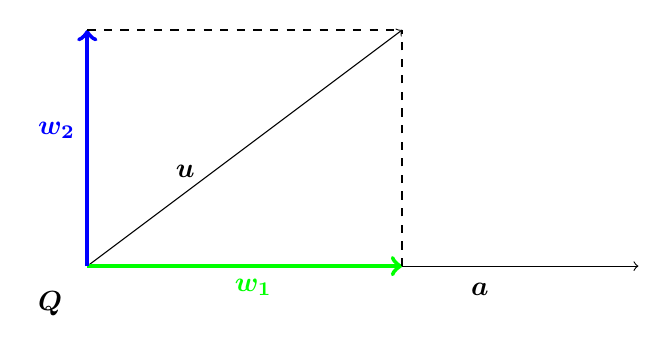
\begin{tikzpicture}
\draw [,black](-2.75, -2.75) node [anchor=south west]{$\boldsymbol{Q}$} [->, black](-2, -2) -- (2, 1) ;
\draw [,black](-1, -1) node[anchor=south west]{$\boldsymbol{u}$};
\draw [->, black](-2, -2) -- (5, -2) ;
\draw [,black](2.75, -2.5) node [anchor=south west]{$\boldsymbol{a}$};
\draw [->, ultra thick, green](-2, -2) -- (2, -2) ;
\draw [->, ultra thick, blue](-2, -2) -- (-2, 1) ;
\draw [, blue] (-2.75, -.5) node [anchor=south west]{$\boldsymbol{w_2}$};
\draw [dashed, thick, black] (-2, 1) -- (2, 1);
\draw [, green] (-.25, -2.5) node [anchor=south west]{$\boldsymbol{w_1}$};
\draw [dashed, thick, black](2, -2) -- (2, 1) ;
%\draw[-, black](-2, -2) -> (1, 2) 
%\draw(-2, -2) --> (3, -2);
\end{tikzpicture} 
\\
Proof
\begin{align*}
k &= \norm{u}\cos(\theta)\\
u \cdot a &= \norm{u}\norm{a}\cos(\theta)\\
k\norm{a} &= \frac{u \cdot a}{\norm{a}} \\
k &= \frac{u \cdot a}{\norm{a}^2}\\
w_1 &= \frac{u \cdot a}{\norm{a}^2} a\\
w_2 &= u - \frac{u\cdot a}{\norm{a}^2} a
\end{align*} 
in a more common notation 
\begin{align*}
proj_au&= \frac{u \cdot a}{\norm{a}^2} a \text{(vector component of $u$ along $a$)}\\
u - proj_au &= u - \frac{u\cdot a}{\norm{a}^2} a \text{(vector component of $u$ orthogonal to $a$)}
\end{align*}
\\
\\
Example

Find the orthogonal projections of the vectors $e_1 = (1, 0)$ and $e_2 = (0, 1)$ on the line $L$
that makes an angle $\theta$ with positive x-axis in $R^2$

\begin{center}
\begin{tikzpicture}
\draw [->] (0, 0) -- (4, 0) node [black, anchor=west] {$e_1$};
\draw [-, blue, dashed] (4, 0)--++(120:2);
\draw [-] (0, 0) -- (30:7) node [black, anchor=south west] {$L$};
\draw [-] (.65, 0.20) node{$\theta$};
\draw [<->] (1, 0) arc (0:30:1) ; %start:stop:radius
\draw [-, black, dotted] (0, 0)--++(300:4);
\draw [-, blue, dashed] (4, 0)--++(210:3.5);
\draw [<->] (.5, -.8) arc (300:360:1) ; %start:stop:radius
\end{tikzpicture}
\end{center}

\begin{center}
\begin{tikzpicture}
\draw [->] (0, 0) -- (4, 0) node [black, anchor=west] {$e_1$};
\draw [-, blue, dashed] (4, 0)--++(120:2);
\draw [-] (0, 0) -- (30:7) node [black, anchor=south west] {$L$};
\draw [-] (.65, 0.20) node{$\theta$};
\draw [<->] (1, 0) arc (0:30:1) ; %start:stop:radius
\draw [-, black, dotted] (0, 0)--++(300:4);
\draw [-, blue, dashed] (4, 0)--++(210:3.5);
\draw [<->] (.5, -.8) arc (300:360:1) ; %start:stop:radius
\draw (.8*4, .5*4) node {$(\cos\theta, \sin\theta)$};
\end{tikzpicture}
\end{center}

From the picture, we know that vector {$(\cos\theta, \sin\theta)$} is in line $L$.
So we have $a = (\cos\theta, \sin\theta)$

\begin{align*}
proj_{(1, 0)}\vec{a} &= \frac{(1, 0)\cdot(\cos\theta, \sin\theta)}{\norm{a}^2}(\cos\theta, \sin\theta)\\
proj_{(1, 0)}\vec{a} &= (\cos^2\theta, \cos\theta\sin\theta)\\
(1, 0) - proj_{(1, 0)}\vec{a} &= (1 - \cos^2\theta, - \cos\theta\sin\theta)\\
(1, 0) - proj_{(1, 0)}\vec{a} &= (\sin^2\theta, - \cos\theta\sin\theta)
\end{align*}


\begin{center}
\begin{tikzpicture}
\draw [->] (0, 0) -- (0, 4) node [black, anchor=south] {$e_1$};
\draw [-] (0, 0) -- (60:7) node [black, anchor=south west] {$L$};
\draw [-] (.15, 0.75) node{$\theta$};
\draw [<->] (0.45, 0.8) arc (0:120:.30) ; %start:stop:radius
\draw [-, blue, dashed] (0, 4) --++ (-30:.5*4);
\draw [-, blue, dashed] (0, 0) -- (150:.5*4); 
\draw (4*.5, 4*.8) node {$(\sin\theta, \cos\theta)$};
\end{tikzpicture}
\end{center}

\begin{center}
\begin{tikzpicture}
\draw 
\draw [-] (0, 0) -- (60:7) node [black, anchor=south west] {$L$};
\end{center}
\end{tikzpicture}

\begin{align*}
proj_{(0, 1)}a &= \frac{(0, 1)\cdot a}{\norm{a}^2}a\\
&= \frac{(0, 1)\cdot (\sin\theta, \cos\theta)}{\norm{a}^2}a\\
&= \cos\theta(\sin\theta, \cos\theta)\\
&= (\cos\theta\sin\theta, \cos^2\theta)\\
\end{align*}

\textbf{The inner product function.} Suppose $a$ is an $n-vector$. We can define scalar-valued
function $f$ of $n-vectors$, given by
\begin{equation}
f(x) = a^Tx = a_1x_1 + a_2x_2+...+a_nx_n
\end{equation}
for any $n-vector x$. This function gives the inner product of its $n-vector$ argument $x$ with
some (fixed) $n-vector$.
\\
\\ 
\textbf{Superposition and linearity}. The inner product function $f$ defined above satisfies
property
\begin{align*}
f(\alpha x +\beta y) &= a^T(\alpha x + \beta y) \\
&= a^T(\alpha x) + a^T(\beta y) \\
&= \alpha(a^Tx) + \beta(a^Ty) \\
&= \alpha f(x) + \beta f(x)
\end{align*}
\\
for all $n-vectors x, y$, and all scalars $\alpha, \beta$. This property is called \textit{superposition}.
 A function that satisfies the superposition property is called \textit{linear}.
\\
\\
\textbf{Superposition equality} is thus
\begin{equation}
f(\alpha x + \beta y) = \alpha f(x) + \beta f(y)
\end{equation}
\\
A function  $ f: \mathbf{R}^n \to \mathbf{R} $ is linear if satisfies
\begin{itemize}
\item \textit{Homogenity.} For any $n$-vector $x$ and any scala $\alpha$, $f(\alpha x) = \alpha f(x)$
\item \textit{Additivity.} For any $n$-vector $x$ and $y$, $f(x + y) = f(x) + f(y)$
\end{itemize}

\textbf{Inner product representation of linear function}
A function is linear if it is defined as inner product of it's argument with some fixed vector.

$f(x) = a^Tx$ for all $x$.
$a^Tx$ is inner product representation of $f$
\\
\\
\textbf{Affine functions}. A linear function plus a constant is called an \textit{affine} function.
A function $f: \mathbf{R} ^n \to \mathbf{R}$ is affine if an only if it can be expressed as $f(x) = a^T x + b$

\end{document}
